\documentclass[14pt]{extbook}
\usepackage{multicol, enumerate, enumitem, hyperref, color, soul, setspace, parskip, fancyhdr} %General Packages
\usepackage{amssymb, amsthm, amsmath, latexsym, units, mathtools} %Math Packages
\everymath{\displaystyle} %All math in Display Style
% Packages with additional options
\usepackage[headsep=0.5cm,headheight=12pt, left=1 in,right= 1 in,top= 1 in,bottom= 1 in]{geometry}
\usepackage[usenames,dvipsnames]{xcolor}
\usepackage{dashrule}  % Package to use the command below to create lines between items
\newcommand{\litem}[1]{\item#1\hspace*{-1cm}\rule{\textwidth}{0.4pt}}
\pagestyle{fancy}
\lhead{Makeup Progress Quiz 3}
\chead{}
\rhead{Version ALL}
\lfoot{1648-1753}
\cfoot{}
\rfoot{Summer C 2021}
\begin{document}

\begin{enumerate}
\litem{
Which of the following functions \textit{could} be the graph below?
\begin{center}
    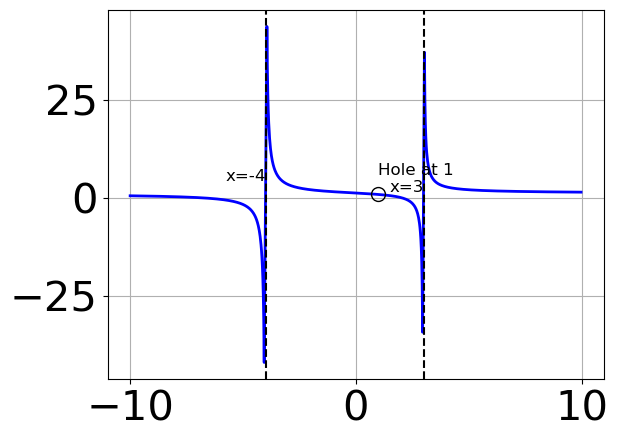
\includegraphics[width=0.5\textwidth]{../Figures/identifyGraphOfRationalFunctionA.png}
\end{center}
\begin{enumerate}[label=\Alph*.]
\item \( f(x)=\frac{x^{3} +10.0 x^{2} +11.0 x -70.0}{x^{3} -13.0 x + 12.0} \)
\item \( f(x)=\frac{x^{3} +4.0 x^{2} -19.0 x + 14.0}{x^{3} -13.0 x + 12.0} \)
\item \( f(x)=\frac{x^{3} + x^{2} -44.0 x -84.0}{x^{3} -13.0 x -12.0} \)
\item \( f(x)=\frac{x^{3} -4.0 x^{2} -19.0 x -14.0}{x^{3} -13.0 x -12.0} \)
\item \( \text{None of the above are possible equations for the graph.} \)

\end{enumerate} }
\litem{
Determine the horizontal and/or oblique asymptotes in the rational function below.\[ f(x) = \frac{12x^{3} -41 x^{2} +44 x -15}{4x^{2} +9 x -9} \]\begin{enumerate}[label=\Alph*.]
\item \( \text{Horizontal Asymptote of } y = -3.0 \text{ and Oblique Asymptote of } y = 3x -17 \)
\item \( \text{Horizontal Asymptote of } y = 3.0  \)
\item \( \text{Oblique Asymptote of } y = 3x -17. \)
\item \( \text{Horizontal Asymptote of } y = 3.0 \text{ and Oblique Asymptote of } y = 3x -17 \)
\item \( \text{Horizontal Asymptote at } y = -3.0 \)

\end{enumerate} }
\litem{
Determine the vertical asymptotes and holes in the rational function below.\[ f(x) = \frac{9x^{3} +9 x^{2} -16 x -16}{12x^{2} -25 x + 12} \]\begin{enumerate}[label=\Alph*.]
\item \( \text{Vertical Asymptote of } x = 0.75 \text{ and hole at } x = 1.333 \)
\item \( \text{Vertical Asymptotes of } x = 0.75 \text{ and } x = -1.333 \text{ with a hole at } x = 1.333 \)
\item \( \text{Vertical Asymptotes of } x = 0.75 \text{ and } x = 1.333 \text{ with no holes.} \)
\item \( \text{Holes at } x = 0.75 \text{ and } x = 1.333 \text{ with no vertical asymptotes.} \)
\item \( \text{Vertical Asymptote of } x = 0.75 \text{ and hole at } x = 1.333 \)

\end{enumerate} }
\litem{
Determine the horizontal and/or oblique asymptotes in the rational function below.\[ f(x) = \frac{6x^{2} -7 x -10}{18x^{3} -87 x^{2} +35 x + 100} \]\begin{enumerate}[label=\Alph*.]
\item \( \text{Horizontal Asymptote of } y = 0.333 \text{ and Oblique Asymptote of } y = 3x -11 \)
\item \( \text{Horizontal Asymptote of } y = 0.333  \)
\item \( \text{Horizontal Asymptote of } y = 0 \)
\item \( \text{Oblique Asymptote of } y = 3x -11. \)
\item \( \text{Horizontal Asymptote at } y = 2.000 \)

\end{enumerate} }
\litem{
Which of the following functions \textit{could} be the graph below?
\begin{center}
    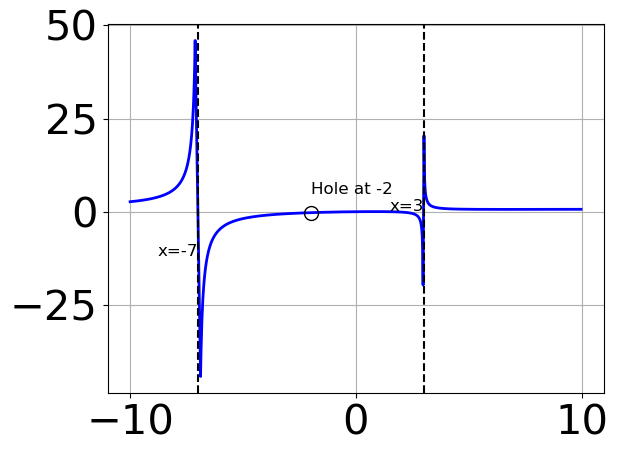
\includegraphics[width=0.5\textwidth]{../Figures/identifyGraphOfRationalFunctionCopyA.png}
\end{center}
\begin{enumerate}[label=\Alph*.]
\item \( f(x)=\frac{x^{3} -6.0 x^{2} +3.0 x + 10.0}{x^{3} +6.0 x^{2} -13.0 x -42.0} \)
\item \( f(x)=\frac{x^{3} -1.0 x^{2} -4.0 x + 4.0}{x^{3} -6.0 x^{2} -13.0 x + 42.0} \)
\item \( f(x)=\frac{x^{3} + x^{2} -4.0 x -4.0}{x^{3} +6.0 x^{2} -13.0 x -42.0} \)
\item \( f(x)=\frac{x^{3} -2.0 x^{2} -5.0 x + 6.0}{x^{3} -6.0 x^{2} -13.0 x + 42.0} \)
\item \( \text{None of the above are possible equations for the graph.} \)

\end{enumerate} }
\litem{
Determine the horizontal and/or oblique asymptotes in the rational function below.\[ f(x) = \frac{6x^{2} -7 x -10}{24x^{3} +74 x^{2} -9 x -45} \]\begin{enumerate}[label=\Alph*.]
\item \( \text{Horizontal Asymptote at } y = 2.000 \)
\item \( \text{Horizontal Asymptote of } y = 0.250  \)
\item \( \text{Horizontal Asymptote of } y = 0.250 \text{ and Oblique Asymptote of } y = 4x + 17 \)
\item \( \text{Horizontal Asymptote of } y = 0 \)
\item \( \text{Oblique Asymptote of } y = 4x + 17. \)

\end{enumerate} }
\litem{
Determine the vertical asymptotes and holes in the rational function below.\[ f(x) = \frac{6x^{3} -43 x^{2} +91 x -60}{9x^{2} -21 x + 10} \]\begin{enumerate}[label=\Alph*.]
\item \( \text{Vertical Asymptotes of } x = 0.667 \text{ and } x = 1.5 \text{ with a hole at } x = 1.667 \)
\item \( \text{Vertical Asymptote of } x = 0.667 \text{ and hole at } x = 1.667 \)
\item \( \text{Vertical Asymptotes of } x = 0.667 \text{ and } x = 1.667 \text{ with no holes.} \)
\item \( \text{Vertical Asymptote of } x = 0.667 \text{ and hole at } x = 1.667 \)
\item \( \text{Holes at } x = 0.667 \text{ and } x = 1.667 \text{ with no vertical asymptotes.} \)

\end{enumerate} }
\litem{
Determine the vertical asymptotes and holes in the rational function below.\[ f(x) = \frac{8x^{3} -2 x^{2} -43 x + 30}{6x^{2} +11 x -10} \]\begin{enumerate}[label=\Alph*.]
\item \( \text{Vertical Asymptote of } x = 1.333 \text{ and hole at } x = -2.5 \)
\item \( \text{Vertical Asymptote of } x = 0.667 \text{ and hole at } x = -2.5 \)
\item \( \text{Vertical Asymptotes of } x = 0.667 \text{ and } x = -2.5 \text{ with no holes.} \)
\item \( \text{Vertical Asymptotes of } x = 0.667 \text{ and } x = 0.75 \text{ with a hole at } x = -2.5 \)
\item \( \text{Holes at } x = 0.667 \text{ and } x = -2.5 \text{ with no vertical asymptotes.} \)

\end{enumerate} }
\litem{
Determine the vertical asymptotes and holes in the rational function below.\[ f(x) = \frac{6x^{3} +17 x^{2} -3 x -20}{6x^{2} +11 x -10} \]\begin{enumerate}[label=\Alph*.]
\item \( \text{Vertical Asymptote of } x = 0.667 \text{ and hole at } x = -2.5 \)
\item \( \text{Vertical Asymptotes of } x = 0.667 \text{ and } x = -2.5 \text{ with no holes.} \)
\item \( \text{Holes at } x = 0.667 \text{ and } x = -2.5 \text{ with no vertical asymptotes.} \)
\item \( \text{Vertical Asymptote of } x = 1.0 \text{ and hole at } x = -2.5 \)
\item \( \text{Vertical Asymptotes of } x = 0.667 \text{ and } x = -1.333 \text{ with a hole at } x = -2.5 \)

\end{enumerate} }
\litem{
Determine the horizontal and/or oblique asymptotes in the rational function below.\[ f(x) = \frac{9x^{3} -9 x^{2} -46 x -24}{3x^{2} +16 x + 16} \]\begin{enumerate}[label=\Alph*.]
\item \( \text{Horizontal Asymptote of } y = 3.0 \text{ and Oblique Asymptote of } y = 3x -19 \)
\item \( \text{Horizontal Asymptote of } y = 3.0  \)
\item \( \text{Oblique Asymptote of } y = 3x -19. \)
\item \( \text{Horizontal Asymptote of } y = -4.0 \text{ and Oblique Asymptote of } y = 3x -19 \)
\item \( \text{Horizontal Asymptote at } y = -4.0 \)

\end{enumerate} }
\litem{
Which of the following functions \textit{could} be the graph below?
\begin{center}
    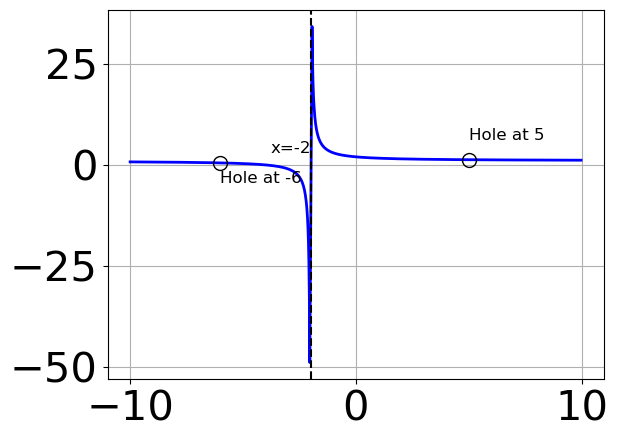
\includegraphics[width=0.5\textwidth]{../Figures/identifyGraphOfRationalFunctionB.png}
\end{center}
\begin{enumerate}[label=\Alph*.]
\item \( f(x)=\frac{x^{3} -5.0 x^{2} -26.0 x + 120.0}{x^{3} -3.0 x^{2} -28.0 x + 60.0} \)
\item \( f(x)=\frac{x^{3} +15.0 x^{2} +72.0 x + 112.0}{x^{3} +3.0 x^{2} -28.0 x -60.0} \)
\item \( f(x)=\frac{x^{3} +5.0 x^{2} -26.0 x -120.0}{x^{3} +3.0 x^{2} -28.0 x -60.0} \)
\item \( f(x)=\frac{x^{3} -6.0 x^{2} + 32.0}{x^{3} -3.0 x^{2} -28.0 x + 60.0} \)
\item \( \text{None of the above are possible equations for the graph.} \)

\end{enumerate} }
\litem{
Determine the horizontal and/or oblique asymptotes in the rational function below.\[ f(x) = \frac{12x^{3} -11 x^{2} -45 x + 50}{3x^{2} -14 x + 15} \]\begin{enumerate}[label=\Alph*.]
\item \( \text{Horizontal Asymptote of } y = 3.0 \text{ and Oblique Asymptote of } y = 4x + 15 \)
\item \( \text{Horizontal Asymptote at } y = 3.0 \)
\item \( \text{Horizontal Asymptote of } y = 4.0 \text{ and Oblique Asymptote of } y = 4x + 15 \)
\item \( \text{Horizontal Asymptote of } y = 4.0  \)
\item \( \text{Oblique Asymptote of } y = 4x + 15. \)

\end{enumerate} }
\litem{
Determine the vertical asymptotes and holes in the rational function below.\[ f(x) = \frac{6x^{3} +7 x^{2} -56 x + 48}{12x^{2} -25 x + 12} \]\begin{enumerate}[label=\Alph*.]
\item \( \text{Vertical Asymptote of } x = 0.5 \text{ and hole at } x = 1.333 \)
\item \( \text{Vertical Asymptotes of } x = 0.75 \text{ and } x = 1.5 \text{ with a hole at } x = 1.333 \)
\item \( \text{Vertical Asymptotes of } x = 0.75 \text{ and } x = 1.333 \text{ with no holes.} \)
\item \( \text{Vertical Asymptote of } x = 0.75 \text{ and hole at } x = 1.333 \)
\item \( \text{Holes at } x = 0.75 \text{ and } x = 1.333 \text{ with no vertical asymptotes.} \)

\end{enumerate} }
\litem{
Determine the horizontal and/or oblique asymptotes in the rational function below.\[ f(x) = \frac{6x^{2} -17 x + 10}{24x^{3} -38 x^{2} -45 x + 50} \]\begin{enumerate}[label=\Alph*.]
\item \( \text{Horizontal Asymptote of } y = 0.250 \text{ and Oblique Asymptote of } y = 4x + 5 \)
\item \( \text{Horizontal Asymptote of } y = 0.250  \)
\item \( \text{Oblique Asymptote of } y = 4x + 5. \)
\item \( \text{Horizontal Asymptote at } y = 2.000 \)
\item \( \text{Horizontal Asymptote of } y = 0 \)

\end{enumerate} }
\litem{
Which of the following functions \textit{could} be the graph below?
\begin{center}
    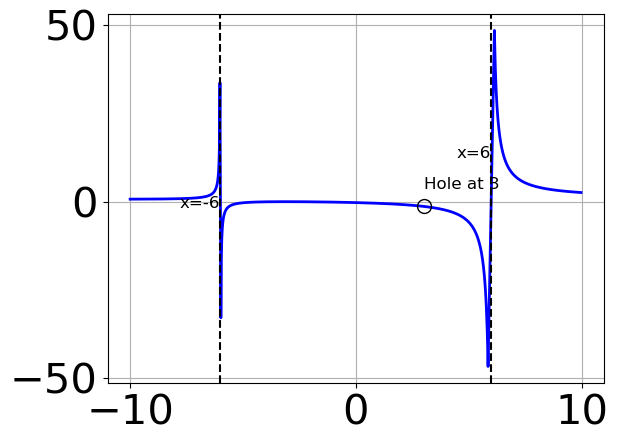
\includegraphics[width=0.5\textwidth]{../Figures/identifyGraphOfRationalFunctionCopyB.png}
\end{center}
\begin{enumerate}[label=\Alph*.]
\item \( f(x)=\frac{x^{3} +9.0 x^{2} +26.0 x + 24.0}{x^{3} -3.0 x^{2} -36.0 x + 108.0} \)
\item \( f(x)=\frac{x^{3} -4.0 x^{2} -4.0 x + 16.0}{x^{3} +3.0 x^{2} -36.0 x -108.0} \)
\item \( f(x)=\frac{x^{3} -3.0 x^{2} -10.0 x + 24.0}{x^{3} +3.0 x^{2} -36.0 x -108.0} \)
\item \( f(x)=\frac{x^{3} +3.0 x^{2} -10.0 x -24.0}{x^{3} -3.0 x^{2} -36.0 x + 108.0} \)
\item \( \text{None of the above are possible equations for the graph.} \)

\end{enumerate} }
\litem{
Determine the horizontal and/or oblique asymptotes in the rational function below.\[ f(x) = \frac{4x^{2} -17 x -15}{24x^{3} +14 x^{2} -23 x -15} \]\begin{enumerate}[label=\Alph*.]
\item \( \text{Horizontal Asymptote of } y = 0 \)
\item \( \text{Horizontal Asymptote of } y = 0.167  \)
\item \( \text{Oblique Asymptote of } y = 6x + 29. \)
\item \( \text{Horizontal Asymptote of } y = 0.167 \text{ and Oblique Asymptote of } y = 6x + 29 \)
\item \( \text{Horizontal Asymptote at } y = 5.000 \)

\end{enumerate} }
\litem{
Determine the vertical asymptotes and holes in the rational function below.\[ f(x) = \frac{16x^{3} -56 x^{2} -47 x + 60}{8x^{2} -18 x + 9} \]\begin{enumerate}[label=\Alph*.]
\item \( \text{Vertical Asymptote of } x = 1.5 \text{ and hole at } x = 0.75 \)
\item \( \text{Holes at } x = 1.5 \text{ and } x = 0.75 \text{ with no vertical asymptotes.} \)
\item \( \text{Vertical Asymptotes of } x = 1.5 \text{ and } x = -1.25 \text{ with a hole at } x = 0.75 \)
\item \( \text{Vertical Asymptotes of } x = 1.5 \text{ and } x = 0.75 \text{ with no holes.} \)
\item \( \text{Vertical Asymptote of } x = 2.0 \text{ and hole at } x = 0.75 \)

\end{enumerate} }
\litem{
Determine the vertical asymptotes and holes in the rational function below.\[ f(x) = \frac{12x^{3} +37 x^{2} -59 x -60}{12x^{2} -5 x -25} \]\begin{enumerate}[label=\Alph*.]
\item \( \text{Holes at } x = -1.25 \text{ and } x = 1.667 \text{ with no vertical asymptotes.} \)
\item \( \text{Vertical Asymptote of } x = 1.0 \text{ and hole at } x = 1.667 \)
\item \( \text{Vertical Asymptote of } x = -1.25 \text{ and hole at } x = 1.667 \)
\item \( \text{Vertical Asymptotes of } x = -1.25 \text{ and } x = -0.75 \text{ with a hole at } x = 1.667 \)
\item \( \text{Vertical Asymptotes of } x = -1.25 \text{ and } x = 1.667 \text{ with no holes.} \)

\end{enumerate} }
\litem{
Determine the vertical asymptotes and holes in the rational function below.\[ f(x) = \frac{8x^{3} -26 x^{2} -33 x + 36}{6x^{2} +19 x + 15} \]\begin{enumerate}[label=\Alph*.]
\item \( \text{Holes at } x = -1.667 \text{ and } x = -1.5 \text{ with no vertical asymptotes.} \)
\item \( \text{Vertical Asymptote of } x = 1.333 \text{ and hole at } x = -1.5 \)
\item \( \text{Vertical Asymptotes of } x = -1.667 \text{ and } x = -1.5 \text{ with no holes.} \)
\item \( \text{Vertical Asymptotes of } x = -1.667 \text{ and } x = 0.75 \text{ with a hole at } x = -1.5 \)
\item \( \text{Vertical Asymptote of } x = -1.667 \text{ and hole at } x = -1.5 \)

\end{enumerate} }
\litem{
Determine the horizontal and/or oblique asymptotes in the rational function below.\[ f(x) = \frac{8x^{3} -10 x^{2} -9 x + 9}{2x^{2} +5 x -12} \]\begin{enumerate}[label=\Alph*.]
\item \( \text{Horizontal Asymptote of } y = 4.0  \)
\item \( \text{Oblique Asymptote of } y = 4x -15. \)
\item \( \text{Horizontal Asymptote at } y = -4.0 \)
\item \( \text{Horizontal Asymptote of } y = -4.0 \text{ and Oblique Asymptote of } y = 4x -15 \)
\item \( \text{Horizontal Asymptote of } y = 4.0 \text{ and Oblique Asymptote of } y = 4x -15 \)

\end{enumerate} }
\litem{
Which of the following functions \textit{could} be the graph below?
\begin{center}
    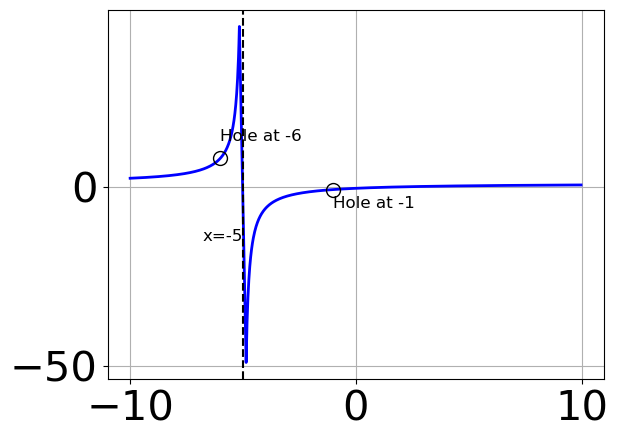
\includegraphics[width=0.5\textwidth]{../Figures/identifyGraphOfRationalFunctionC.png}
\end{center}
\begin{enumerate}[label=\Alph*.]
\item \( f(x)=\frac{x^{3} +7.0 x^{2} +14.0 x + 8.0}{x^{3} -12.0 x^{2} +41.0 x -30.0} \)
\item \( f(x)=\frac{x^{3} -9.0 x^{2} +20.0 x -12.0}{x^{3} +12.0 x^{2} +41.0 x + 30.0} \)
\item \( f(x)=\frac{x^{3} +5.0 x^{2} -8.0 x -12.0}{x^{3} +12.0 x^{2} +41.0 x + 30.0} \)
\item \( f(x)=\frac{x^{3} -5.0 x^{2} -8.0 x + 12.0}{x^{3} -12.0 x^{2} +41.0 x -30.0} \)
\item \( \text{None of the above are possible equations for the graph.} \)

\end{enumerate} }
\litem{
Determine the horizontal and/or oblique asymptotes in the rational function below.\[ f(x) = \frac{9x^{3} -39 x^{2} +52 x -20}{3x^{2} -14 x + 15} \]\begin{enumerate}[label=\Alph*.]
\item \( \text{Horizontal Asymptote of } y = 3.0 \text{ and Oblique Asymptote of } y = 3x + 1 \)
\item \( \text{Horizontal Asymptote of } y = 3.0  \)
\item \( \text{Horizontal Asymptote of } y = 3.0 \text{ and Oblique Asymptote of } y = 3x + 1 \)
\item \( \text{Horizontal Asymptote at } y = 3.0 \)
\item \( \text{Oblique Asymptote of } y = 3x + 1. \)

\end{enumerate} }
\litem{
Determine the vertical asymptotes and holes in the rational function below.\[ f(x) = \frac{12x^{3} -7 x^{2} -72 x -45}{6x^{2} -5 x -25} \]\begin{enumerate}[label=\Alph*.]
\item \( \text{Vertical Asymptotes of } x = 2.5 \text{ and } x = -0.75 \text{ with a hole at } x = -1.667 \)
\item \( \text{Vertical Asymptotes of } x = 2.5 \text{ and } x = -1.667 \text{ with no holes.} \)
\item \( \text{Vertical Asymptote of } x = 2.0 \text{ and hole at } x = -1.667 \)
\item \( \text{Holes at } x = 2.5 \text{ and } x = -1.667 \text{ with no vertical asymptotes.} \)
\item \( \text{Vertical Asymptote of } x = 2.5 \text{ and hole at } x = -1.667 \)

\end{enumerate} }
\litem{
Determine the horizontal and/or oblique asymptotes in the rational function below.\[ f(x) = \frac{3x^{2} +11 x -20}{9x^{3} -63 x^{2} +128 x -80} \]\begin{enumerate}[label=\Alph*.]
\item \( \text{Oblique Asymptote of } y = 3x -32. \)
\item \( \text{Horizontal Asymptote at } y = -5.000 \)
\item \( \text{Horizontal Asymptote of } y = 0.333  \)
\item \( \text{Horizontal Asymptote of } y = 0.333 \text{ and Oblique Asymptote of } y = 3x -32 \)
\item \( \text{Horizontal Asymptote of } y = 0 \)

\end{enumerate} }
\litem{
Which of the following functions \textit{could} be the graph below?
\begin{center}
    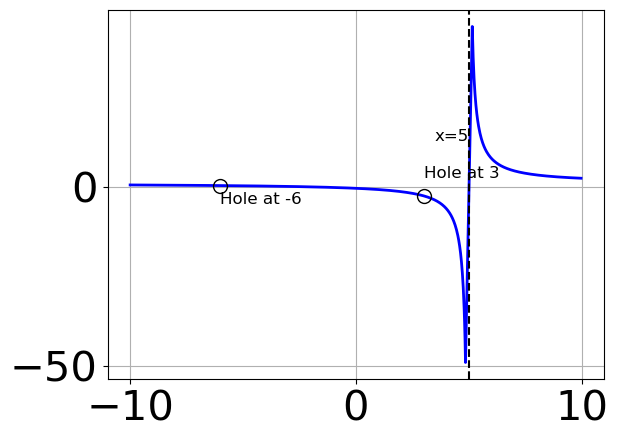
\includegraphics[width=0.5\textwidth]{../Figures/identifyGraphOfRationalFunctionCopyC.png}
\end{center}
\begin{enumerate}[label=\Alph*.]
\item \( f(x)=\frac{x^{3} +5.0 x^{2} -12.0 x -36.0}{x^{3} -2.0 x^{2} -33.0 x + 90.0} \)
\item \( f(x)=\frac{x^{3} -4.0 x^{2} -4.0 x + 16.0}{x^{3} +2.0 x^{2} -33.0 x -90.0} \)
\item \( f(x)=\frac{x^{3} +6.0 x^{2} +3.0 x -10.0}{x^{3} -2.0 x^{2} -33.0 x + 90.0} \)
\item \( f(x)=\frac{x^{3} -5.0 x^{2} -12.0 x + 36.0}{x^{3} +2.0 x^{2} -33.0 x -90.0} \)
\item \( \text{None of the above are possible equations for the graph.} \)

\end{enumerate} }
\litem{
Determine the horizontal and/or oblique asymptotes in the rational function below.\[ f(x) = \frac{4x^{2} +17 x -15}{20x^{3} +49 x^{2} -112 x + 48} \]\begin{enumerate}[label=\Alph*.]
\item \( \text{Horizontal Asymptote at } y = -5.000 \)
\item \( \text{Horizontal Asymptote of } y = 0 \)
\item \( \text{Oblique Asymptote of } y = 5x -9. \)
\item \( \text{Horizontal Asymptote of } y = 0.200 \text{ and Oblique Asymptote of } y = 5x -9 \)
\item \( \text{Horizontal Asymptote of } y = 0.200  \)

\end{enumerate} }
\litem{
Determine the vertical asymptotes and holes in the rational function below.\[ f(x) = \frac{12x^{3} -19 x^{2} -45 x -18}{12x^{2} +25 x + 12} \]\begin{enumerate}[label=\Alph*.]
\item \( \text{Vertical Asymptotes of } x = -1.333 \text{ and } x = -0.667 \text{ with a hole at } x = -0.75 \)
\item \( \text{Vertical Asymptotes of } x = -1.333 \text{ and } x = -0.75 \text{ with no holes.} \)
\item \( \text{Vertical Asymptote of } x = -1.333 \text{ and hole at } x = -0.75 \)
\item \( \text{Holes at } x = -1.333 \text{ and } x = -0.75 \text{ with no vertical asymptotes.} \)
\item \( \text{Vertical Asymptote of } x = 1.0 \text{ and hole at } x = -0.75 \)

\end{enumerate} }
\litem{
Determine the vertical asymptotes and holes in the rational function below.\[ f(x) = \frac{4x^{3} -12 x^{2} -7 x + 30}{6x^{2} -11 x -10} \]\begin{enumerate}[label=\Alph*.]
\item \( \text{Vertical Asymptotes of } x = -0.667 \text{ and } x = 2.5 \text{ with no holes.} \)
\item \( \text{Vertical Asymptotes of } x = -0.667 \text{ and } x = -1.5 \text{ with a hole at } x = 2.5 \)
\item \( \text{Vertical Asymptote of } x = -0.667 \text{ and hole at } x = 2.5 \)
\item \( \text{Vertical Asymptote of } x = 0.667 \text{ and hole at } x = 2.5 \)
\item \( \text{Holes at } x = -0.667 \text{ and } x = 2.5 \text{ with no vertical asymptotes.} \)

\end{enumerate} }
\litem{
Determine the vertical asymptotes and holes in the rational function below.\[ f(x) = \frac{6x^{3} +23 x^{2} -10 x -75}{4x^{2} +16 x + 15} \]\begin{enumerate}[label=\Alph*.]
\item \( \text{Vertical Asymptotes of } x = -1.5 \text{ and } x = -2.5 \text{ with no holes.} \)
\item \( \text{Holes at } x = -1.5 \text{ and } x = -2.5 \text{ with no vertical asymptotes.} \)
\item \( \text{Vertical Asymptotes of } x = -1.5 \text{ and } x = 1.667 \text{ with a hole at } x = -2.5 \)
\item \( \text{Vertical Asymptote of } x = 1.5 \text{ and hole at } x = -2.5 \)
\item \( \text{Vertical Asymptote of } x = -1.5 \text{ and hole at } x = -2.5 \)

\end{enumerate} }
\litem{
Determine the horizontal and/or oblique asymptotes in the rational function below.\[ f(x) = \frac{8x^{3} +26 x^{2} -5 x -50}{4x^{2} -25 x + 25} \]\begin{enumerate}[label=\Alph*.]
\item \( \text{Horizontal Asymptote at } y = 5.0 \)
\item \( \text{Horizontal Asymptote of } y = 2.0  \)
\item \( \text{Horizontal Asymptote of } y = 2.0 \text{ and Oblique Asymptote of } y = 2x + 19 \)
\item \( \text{Horizontal Asymptote of } y = 5.0 \text{ and Oblique Asymptote of } y = 2x + 19 \)
\item \( \text{Oblique Asymptote of } y = 2x + 19. \)

\end{enumerate} }
\end{enumerate}

\end{document}